
\documentclass[12pt]{article}
\usepackage[utf8]{inputenc}
\usepackage[T1]{fontenc}
\usepackage[spanish]{babel}
\usepackage{amsmath,amssymb,mathtools}
\usepackage{graphicx}
\usepackage{float}
\usepackage[margin=1in]{geometry}
\usepackage{parskip}
\usepackage{microtype}





\title{Dinámicas del gasto público en salud en el Perú: evidencia de quiebres estructurales y análisis de serie de tiempo (1980-2022)}
\author{Luciano Díaz Tejada}
\date{Lima, Julio 2025}

\begin{document}
\maketitle
\section{Introducción}

Hablar del gasto público en salud en el Perú implica enfrentar una de las paradojas más complejas del país: aunque se reconoce su importancia, durante décadas ha sido relegado en la práctica. A pesar que desde los noventa el país ha vivido largos periodos de crecimiento económico, la inversión estatal en salud no ha seguido el mismo ritmo. En 2022, por ejemplo, el gasto público en salud apenas alcanzó el 3.91\% del PBI, muy por debajo del 6\% que recomienda la Organización Panamericana de la Salud (Organización Panamericana de la Salud [OPS], 2014). La pandemia de COVID-19 no hizo más que desnudar esa fragilidad: mostró que los hospitales colapsan rápido, que la infraestructura es desigual, y que la falta de planificación pasa factura cuando más se necesita.


Este trabajo parte de una pregunta que muchos se han hecho, pero que rara vez se ha abordado con herramientas rigurosas: ¿por qué, a pesar del crecimiento económico sostenido, el Perú no ha logrado consolidar una política pública de salud ambiciosa y estable? Para responderla, se vincula la historia económica con análisis estadístico. Aplicamos pruebas ADF con variables dicotómicas, modelos en logaritmos, y el test de Bai y Perron (2003) para identificar quiebres estructurales en la serie de gasto del periodo 1980-2022. Los resultados sugieren tres grandes momentos: un estancamiento antes de 1992, una fuerte expansión hasta 2009, y una etapa de crecimiento más moderado posteriormente. La hipótesis es clara: el gasto público en salud no ha respondido solo a criterios técnicos o demográficos, sino a shocks, restricciones fiscales y decisiones políticas que, en muchas ocasiones, han sido reactivas. Mirar con lupa esos momentos —dónde se acelera el gasto, cuándo se estanca, y por qué— permite entender mejor cómo llegamos hasta aquí y qué obstáculos hay que sortear para avanzar.

\bigskip
\bigskip
\section{Revisión de la literatura}

\subsection{Crisis, reformas y trayectoria del gasto}

Los años ochenta fueron una época crítica para el Perú. El Estado enfrentó una combinación devastadora: crisis de deuda, hiperinflación y violencia política. En ese contexto, mantener un sistema de salud funcional fue simplemente inviable. Contreras y Cueto (2007) muestran cómo estas crisis redujeron el gasto público en salud a niveles mínimos. El análisis econométrico de este estudio respalda esa lectura: antes de 1992, no se observa una tendencia significativa de crecimiento en el gasto logarítmico, lo cual indica una parálisis institucional más que una decisión presupuestal deliberada.


El giro se produce en 1992. Las reformas estructurales posteriores a la hiperinflación, como las que describe Gonzales de Olarte (1998), marcan un cambio en el enfoque fiscal. Empieza una etapa de crecimiento sostenido del gasto en salud —con una tasa promedio del 11.4\% anual en términos logaritmos—, que se explica tanto por la recuperación de ingresos fiscales como por una necesidad acumulada. No significa que el Estado priorizara la salud como política de fondo, pero sí que ya tenía margen para moverse. Durante este periodo, hubo avances: la Organización para la Cooperación y el Desarrollo Económico (OCDE, 2017) documenta una ampliación de la cobertura, aunque advierten que los problemas estructurales —como la fragmentación institucional— seguían presentes. Jaramillo y Parodi (2003) también destacan cómo la rigidez de las reglas fiscales dificultaba una planificación ambiciosa. El modelo econométrico muestra que, sin controlar por quiebres, los residuos presentan una gran volatilidad, lo cual sugiere que los aumentos de gasto fueron más respuestas puntuales que una política de Estado.

\subsection{Fragmentación institucional y capacidad limitada}

La estructura del sistema de salud es otro gran desafío. Mendoza-Arana et al. (2018) describen un panorama institucional disperso: el Ministerio de Salud (MINSA), EsSalud, sanidad militar y gobiernos subnacionales operan con poca coordinación, sin una autoridad rectora clara. La OCDE (2025), desde una perspectiva externa, lo confirma: la fragmentación limita tanto la eficiencia como la capacidad de respuesta frente a crisis, lo cual se convierte en un obstáculo estructural. Esto explica por qué, incluso cuando aumentó el presupuesto entre 1992 y 2009, los resultados en cobertura efectiva y equidad fueron modestos. 


EsSalud, entre el 2013 y 2022, continuó mostrando grandes brechas entre regiones, falta de personal médico y déficits crónicos de infraestructura. Además, el estudio de Coaquira y Vilca (2023), que emplea el coeficiente de Gini para medir la desigualdad en la ejecución del gasto a nivel provincial, destaca las significativas las brechas territoriales significativas. Esto nos sugiere que tener más recursos no es suficiente si no existe capacidad institucional para ejecutarlos adecuadamente.

\subsection{Crisis sanitarias y respuestas reactivas}

Las crisis han sido puntos de quiebre, pero rara vez motores de reforma profunda. La epidemia del cólera en 1991 obligó a reaccionar, igual que la pandemia de COVID-19 en 2020. En ambos casos, hubo picos de gasto, pero no transformaciones sostenidas (Mendoza-Arana et al., 2018). El modelo de quiebres múltiples detecta otro punto de inflexión en 2009, que coincide con la implementación del Aseguramiento Universal en Salud y la epidemia de H1N1. A partir de ese momento, el modelo incorpora una pendiente adicional al ritmo de crecimiento del gasto. Es decir, no hay una desaceleración, sino una aceleración moderada: se añade un crecimiento de 3.3\% anual (en logaritmos) al ritmo ya existente desde 1992. Esto eleva el crecimiento total a aproximadamente 14.7\% anual en logaritmos desde 2009, una señal de continuidad, no de ruptura.

Los datos de ENSUSALUD posteriores a 2009 muestran pequeñas mejoras en percepción de calidad, pero también reflejan que muchas falencias estructurales siguen sin resolverse. La meta del 6\% del PBI en gasto público en salud, propuesta por la OPS (2014), sigue siendo eso: una meta pendiente que aún no se ha alcanzado. Las grandes crisis sanitarias han funcionado en el Perú como catalizadores de gasto, pero rara vez como puntos de inflexión institucional. La epidemia del cólera en 1991 o la pandemia de COVID-19 en 2020 sirvieron para inyectar recursos, pero no para transformar el sistema de fondo (Mendoza-Arana et al., 2018).

\subsection{Salud pública y estudios cuantitativos}

La salud pública, según Winslow (1920), Acheson (1988) y la OMS (1998), no se limita a la atención médica; es una apuesta colectiva por la prevención, el bienestar y la equidad. Analizar cómo se financia revela qué tanto —y cómo— un Estado prioriza ese bienestar. En otros países, el tema ha sido abordado con herramientas econométricas. 

En China, Zheng et al. (2020) usaron modelos ARIMA para prever la evolución del gasto. En Turquía, Atilgan et al. (2016) e Ilgun et al. (2023) analizaron cómo la inflación, el ingreso y las reformas afectan el gasto en salud. En Pakistán, Ullah et al. (2021) emplearon un enfoque similar. En el Perú, en cambio, hay pocos estudios que combinen técnicas estadísticas con una lectura de largo plazo del gasto en salud. Este trabajo busca llenar ese vacío: aplicando pruebas ADF con variables dicotómicas, transformaciones log-lineales y modelos de quiebres múltiples, se identifican momentos clave en la trayectoria del gasto y se los conecta con cambios institucionales. Entender esos ciclos es crucial si se quiere evitar que los errores del pasado se repitan.

\bigskip
\bigskip
\bigskip
\bigskip
\bigskip
\bigskip
\bigskip
\bigskip
\bigskip
\section{Metodología}

Para el análisis del gasto público en salud, se presentaron dos problemas fundamentales. En primer lugar, antes de 1997, el sistema de salud peruano estaba fragmentado en tres subsistemas públicos separados: el Seguro Social de Salud, administrado por el entonces Instituto Peruano de Seguridad Social (IPSS, hoy EsSalud); los servicios de salud a cargo del Ministerio de Salud (MINSA); y el sistema de salud de las Fuerzas Armadas y la Policía Nacional. Esta estructura cambiaría a partir de 1997, cuando estos componentes comenzaron a ser considerados conjuntamente dentro del gasto público en salud (Comisión Económica para América Latina y el Caribe [CEPAL] \& OPS, 2013).

No es posible —o al menos es sumamente difícil— acceder a datos detallados sobre los gastos del IPSS antes de esa fecha, debido a su naturaleza institucional. Este instituto funcionaba como un organismo autónomo y descentralizado, con presupuesto propio y fuera del control directo del Tesoro Público. Su financiamiento provenía principalmente de un esquema tripartito de aportes (trabajadores, empleadores y Estado), lo cual lo alejaba de los esquemas tradicionales de presupuestación del gobierno general (CEPAL \& OPS, 2013).

Además, hasta mediados de los años noventa, el presupuesto público peruano se organizaba por entidad ejecutora y no por función. Esta estructura dificulta la posibilidad de consolidar adecuadamente el gasto público en sectores específicos, como el de salud (Ministerio de Economía y Finanzas [MEF], 2020). Recién con la implementación de la Clasificación Funcional Programática, introducida en el marco de la reforma del sistema presupuestario en 1997, se empezó a integrar de manera sistemática el gasto ejecutado por el MINSA, EsSalud y otras entidades bajo la categoría de “salud pública” (OPS, 2008).

A ello se sumaban debilidades institucionales como la falta de transparencia, la escasa fiscalización y la ausencia de sistemas de información interoperables, en un contexto en que el Estado peruano aún no había avanzado hacia la digitalización ni adoptado prácticas modernas de gestión fiscal. Antes de la existencia de las Cuentas Nacionales de Salud, las estadísticas fiscales eran fragmentadas, incompletas y, en muchos casos, no auditadas (OPS, 2012). 

Esta es la razón por la cual se decidió usar como referencia solamente el gasto del Gobierno Central, dado que solo se encontró información disponible para este sector. Para años posteriores a 1997, se suprimió al gasto público en salud, los sistemas de seguro social y los pagos al servicio de salud de la policía y el ejército, pues esto no se registra previo a 1997. En otras palabras, se optó por considerar solamente el gasto del MINSA y de las regiones. Sin embargo, este método no altera realmente las predicciones de la serie creada, puesto que el gasto en servicios de salud desde 1996 ha sido relativamente estable (MINSA \& OMS, 2015). Ello puede notarse en la gran similitud que tienen los gráficos 1 y 2. 

El segundo problema estriba en las distintas bases de datos con las cuales se recabó información. Para los años de 1980 a 1991, se recurrió al estudio de Portocarrero (1992), dado que esquematiza la contabilidad del gasto del Estado del seguro social, y aparece el gasto del Estado, pues, en salud. De 1991 a 1995, se utilizó la información de Cruz (1998), quien también se basa en las cifras del MINSA. Entre 1995 y 2000, se recurrió a la información de las Cuentas Nacionales del MINSA (2015). Y, finalmente, de 2000 a 2022, se recurrió a la información de la Organización Mundial de la Salud (2025). 

La elección de estas bases de datos no ha sido arbitraria: debido a la escasez de fuentes primarias acerca de los gastos de los años seleccionados, se eligieron fuentes secundarias (para los casos previos a 1995). En los casos posteriores, se prefirió la información de la Organización Mundial de la Salud. Esto, debido a que, por un lado, el gasto directo de las personas no es recogido completamente por el MINSA, lo que genera que el gasto se esté sobreestimado al subestimar el gasto privado (en porcentaje) (Banco Mundial, 2016); por otro lado, “El sistema de información de salud de Perú no está estandarizado entre subsistemas y es difícil conectar datos personales de salud entre entes. Esto impide medir actividades, calidad o resultados de forma nacional” (OCDE, 2017). 

Si bien tanto la data previa a los 2000 puede estar subestimada por lo mismo que no está estandarizada, ello no impide que se pueda formar una serie de tiempo, como la que está en el gráfico 2. 

\bigskip


\begin{figure}[H]
\centering{Gráfico 1: Gasto público total en salud entre 1996 y 2022 en miles de soles del 2007}
\par\vspace{0.8em}
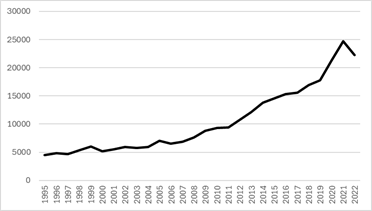
\includegraphics[width=0.5\linewidth]{Imagen2.png}

{\footnotesize Elaboración propia. Información extraída de OMS (2025) y MINSA (2012).}
\end{figure}



\begin{figure}[H]
\centering{Gráfico 2: Gasto del Gobierno Central entre 1980 y 2022 en miles de soles del 2007}
\par\vspace{0.8em}
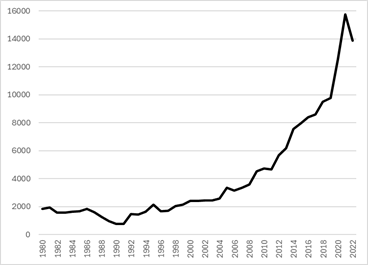
\includegraphics[width=0.5\linewidth]{Imagen3.png}

{\footnotesize Elaboración propia. Información extraída de OMS (2025) y MINSA (2012).}
\end{figure}

Con la información clara, es posible manipularla de tal modo que pueda ofrecernos respuestas sobre aquellos procesos detrás de los gastos en salud a través de los años. Con el fin de reducir la varianza, y sin pérdida de generalidad, se procedió a log-linealizar los valores para cada valor de la tabla, de modo que se obtiene el siguiente gráfico. 

\bigskip
\bigskip
\bigskip

\begin{figure}[H]
\centering{Gráfico 3: Gasto del Gobierno Central log-linealizado entre 1980 y 2022 en miles de soles del 2007}
\par\vspace{0.8em}
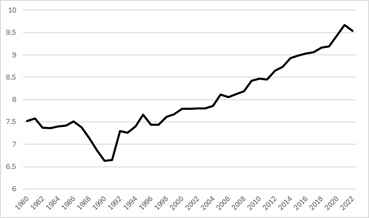
\includegraphics[width=0.5\linewidth]{Imagen4.png}

{\footnotesize Elaboración propia. Información extraída de Portocarrero, (1992), Cruz (1998), MINSA (2012) y OMS (2025).}
\end{figure}

Dado que se trata de una serie de tiempo, es posible expresar la forma funcional del gasto en salud como un proceso autorregresivo. Para estimar su forma óptima, es necesario seguir el procedimiento establecido por Box \& Jenkins (1976). Así, observando la serie, es obvio que va a haber una tendencia involucrada. De este modo, la primera ecuación a estimar tendría la siguiente forma: 

\begin{center}
\title{Ecuación 1: Forma funcional del Gasto Público}
\end{center}
\begin{equation}
gastopublico_{t}= \beta + \gamma t + \sum_{i=1}^{p} \delta_{i}gastopublico_{t-i} + \alpha^{\top} X + \epsilon_{i}
\end{equation}

Ahora bien, las pruebas de correlación sugieren la posible presencia de raíz unitaria, lo cual se confirma al aplicar la prueba de Dickley-Fuller aumentada (ADF), cuyos resultados pueden observarse en el Anexo 3. Debido a ello, se procede a utilizar la prueba tanto de Zivot-Andrews como la de Bai-Perron con el fin de volver la serie estacionaria. Los resultados muestran tres quiebres estructurales: la prueba de Zivot-Andrews identifica un quiebre en 2004, mientras que la prueba de Bai-Perron detecta rupturas en 1992 y 2009. Los tres llegan a ser significativos (ver Anexo 4 y 5). Posteriormente, con el fin de analizar la estacionalidad del modelo, se aplicaron funciones trigonométricas de Fourier, siguiendo la metodología propuesta por Seminario (2006), lo cual permite un control más flexible de la estacionalidad. Sin embargo, los resultados no fueron estadísticamente significativos (ver Anexo 6). Esto es, el gasto público en el Perú no tiene un comportamiento cíclico. 

Con el objetivo de ver si permiten solucionar el problema de raíz unitaria, se procederá a correr la regresión propia de la prueba ADF, el cual tiene la siguiente forma: 

\begin{center}
Ecuación 2: Test Dickley Fuller con la presencia de un quiebre estructural (Zivot-Andrews)    
\end{center}
\begin{equation}
\Delta gastopublic{o}_{t} = \beta + \gamma t + \rho \, gastopublic{o}_{t-1} + \sum_{i=1}^{p-1} \delta_{i} \, \Delta gastopublic{o}_{t-i} + \theta_{1} D_{04} + \varepsilon_{i}
\end{equation}
\begin{center}
Donde: 
\end{center}
\begin{equation*}
D_{92}=1,\ si\ t>1992\ y\ 0\ d.o.m
\end{equation*}
\begin{equation*}
D_{09}=1,\ si\ t>2009\ y\ 0\ d.o.m
\end{equation*}

\bigskip
\begin{center}
Ecuación 3: Test Dickley Fuller con la presencia de varios quiebre estructural (Bai-Perron)
\end{center}
\begin{equation}
\Delta gastopublic{o}_{t} = \beta + \gamma t + \rho \, gastopublic{o}_{t-1} + \sum_{i=1}^{p-1} \delta_{i} \, \Delta gastopublic{o}_{t-i} + \theta_{1} D_{92} + \theta_{2} D_{09} + \varepsilon_{i}
\end{equation}
\begin{center}
Donde: 
\end{center}
\begin{equation*}
D_{92}=1,\ si\ t>1992\ y\ 0\ d.o.m
\end{equation*}
\begin{equation*}
D_{09}=1,\ si\ t>2009\ y\ 0\ d.o.m
\end{equation*}

Téngase en cuenta que la elección del número de rezagos que irá dentro de la sumatoria va a estar definido por aquel valor que minimice los criterios de Schwartz y de Akaike. 

Posteriormente, se procede a estimar la función de residuos. Con el objetivo de verificar si los quiebres estructurales identificados son suficientes para garantizar la estacionariedad del modelo, se complementa el análisis aplicando el filtro de Hodrick-Prescott. Esta prueba es importante ya que permite descomponer el componente tendencial del componente cíclico, de modo que permite rastrear aquellos momentos vinculados con gastos en salud a la baja (negativos) y gastos en salud al alta (positivos). 

\section{Resultados}

Como se mencionó anteriormente, los Anexos 4 y 5 presentan los resultados de quiebres estructurales identificados mediante las pruebas de Zivot-Andrews y Bai-Perron, respectivamente. Dado que ambas pruebas detectan rupturas en momentos distintos, surge la pregunta: ¿cuál debe utilizarse? Pues aquel que, incluyéndolo en la prueba de Augmented Dickley-Fuller, permita volver estacionaria la serie. Las pruebas correspondientes pueden verse en los anexos 7 y 8. De este modo, los resultados del test Zivot-Andrews de 2004 resultan no volver estacionaria la serie; en cambio, los resultados de Bai-Perron si lo hacen. Así, se considerarán en adelante meramente estos resultados. De este modo, a partir de este punto, se trabajará con estos resultados para la transformación de la serie. 

\bigskip
\bigskip
\bigskip
\bigskip
\bigskip
\bigskip
\bigskip
El número de rezagos que minimiza el valor de Schwartz y Akaike es 0, por lo que la ecuación a estimar tendrá la siguiente forma: 

\begin{center}
Ecuación 4: Test Dickley Fuller a estimar
\end{center}
\begin{equation}
\Delta gastopublico_t=\beta+\gamma t+\rho gastopublico_{t-1}+\theta_1\ D_{92}+\theta_2\ D_{09}\ +\epsilon_i
\end{equation}


Como se mencionó anteriormente, los resultados pueden observarse en el Anexo 8. Interpretando los resultados, tanto 1992 como el 2009 son determinantes en el aumento del gasto público en salud. Con esta nueva información, y dado que no es necesario diferenciar la serie para volverla estacionaria, se evalúa una nueva ecuación, de la siguiente forma

\begin{center}
Ecuación 5: Ecuación final a estimar  
\end{center}
\begin{equation}
gastopublico_t=\beta+\gamma t+\rho gastopublico_{t-1}+ \theta_1 D_{92}+\theta_2 D_{09} + \theta_3 DT_{92}+θ_4DT_{09}+ \epsilon_i
\end{equation}
Donde: 
\begin{equation*}
{DT}_{92}=t,\ si\ t>1992\ y\ 0\ d.o.m
\end{equation*}
\begin{equation*}
{DT}_{09}=t,\ si\ t>2009\ y\ 0\ d.o.m
\end{equation*}

Dado que la variable dicotómica correspondiente al quiebre de 2009 no resulta estadísticamente significativa, se concluye que el cambio observado en ese año se refleja principalmente en la pendiente de la serie. Con base en ello, se obtienen los resultados finales que se presentan en la Tabla 1.

El modelo econométrico estimado permite entender con mayor claridad cómo ha cambiado el gasto público en salud en el Perú en las últimas décadas. Uno de los primeros elementos a destacar es la existencia de inercia en la serie temporal: el coeficiente del rezago del gasto (SERIES02(-1)), que está en logaritmos, es de 0.28. Esto significa que, si el gasto crece un 1\% en un año, al año siguiente tiende a incrementarse en un 0.28\% adicional, por simple arrastre. Sin embargo, lo más interesante aparece cuando se analiza la tendencia. Antes de 1992, el gasto seguía una pendiente negativa fuerte: el coeficiente de tendencia (@TREND) es de −0.067, lo que equivale a una caída promedio anual del 6.7\%. Este resultado respalda lo señalado por otros estudios sobre el colapso del aparato estatal durante la década de 1980: un sistema de salud paralizado, sin margen ni capacidad de respuesta. 

\begin{figure}[H]
\centering{Tabla 1: Resultados de la regresión}
\par\vspace{0.8em}

\includegraphics{Imagen5.png}
{\footnotesize Elaboración propia.}
\end{figure}

En 1992, se produce un cambio significativo. El modelo detecta un salto inmediato en el nivel del gasto, representado por la variable dicotómica D92, cuyo coeficiente de 0.399, que equivale a un incremento de casi 49\% en ese año. No obstante, el cambio no se limita a un aumento puntual: desde ese momento, la pendiente cambia por completo. A partir de 1992, el gasto público en salud comienza a crecer en promedio 11.4\% por año, como muestra el coeficiente positivo de la variable TREND92 (0.108). Este comportamiento marca un quiebre estructural en la trayectoria del gasto, en contraste con la tendencia decreciente observada durante los años previos.

Posteriormente, en 2009, el modelo detecta otro quiebre: la pendiente vuelve a modificarse, esta vez con un coeficiente adicional de 0.0327. Eso implica que desde 2009 el ritmo de crecimiento del gasto se acelera todavía más: a los 11.4\% que ya venían desde 1992, se le suman 3.3\% anuales adicionales. No se trata, entonces, de una desaceleración, sino de una intensificación del crecimiento. Así, el gasto público en salud ha seguido una trayectoria acumulativa, con dos puntos clave —1992 y 2009— que marcan cambios profundos en su dinámica. Estos resultados no son solo números: ayudan a entender cómo y cuándo el Estado empezó a invertir más, y también qué tanto ha logrado sostener ese esfuerzo.

Finalmente, se presenta la prueba de correlación de errores utilizando el estadístico de Liung-Box, donde se ve que los errores no están correlacionados entre sí, lo que implica que el término de perturbación se comporta como ruido blanco.

\begin{figure}[H]
\centering{Tabla 2: Correlograma de los Q-statistics}
\par\vspace{0.8em}
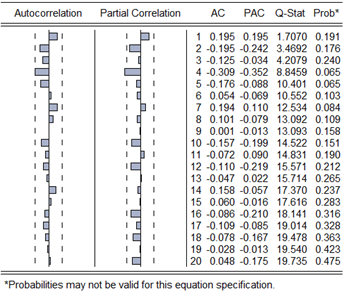
\includegraphics{Imagen6.png}

{\footnotesize Elaboración propia.}
\end{figure}

\begin{figure}[H]
\centering{Gráfico 4: Evolución de los residuos}
\par\vspace{0.8em}
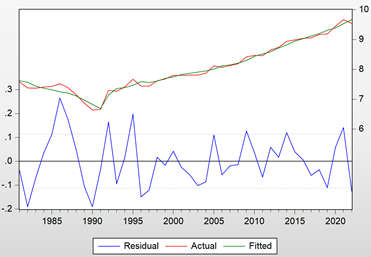
\includegraphics{Imagen7.png}

{\footnotesize Elaboración propia.}
\end{figure}

\bigskip
\bigskip
\bigskip
\bigskip
\bigskip
\bigskip
\bigskip
\bigskip
\bigskip
\bigskip
\bigskip
\bigskip
\bigskip
\bigskip
\bigskip
\bigskip

Como los términos de perturbación se comportan como un ruido blanco, y dado que la serie se ha vuelto estacionaria, entonces tanto 1992 como 2009 son años clave en el análisis de la serie de tiempo. Con el fin de analizar estos resultados más detenidamente, se realizó un filtro de Holdrick-Prescott, de modo que se tiene lo siguiente:

\begin{figure}[H]
\centering{Gráfico 5: Filtro de Hodrick-Prescott sobre la serie de tiempo}
\par\vspace{0.8em}
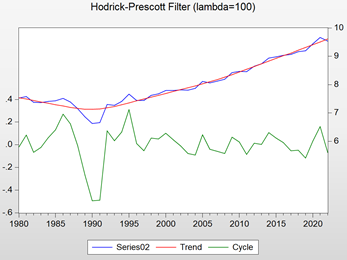
\includegraphics{Imagen8.png}

{\footnotesize Elaboración propia.}
\end{figure}

Donde se confirma que, hasta 1992, la tendencia del gasto era decreciente (-0.0671, en promedio), mientras que después, se hace positiva. En el caso del año 2009, es posible observar que la tendencia “crece más”; ello es explicado en el modelo de arriba por el quiebre en tendencia de este año. En suma, el análisis dinámico del gasto público real en el Perú revela tres etapas claramente diferenciadas. Antes de 1992, la trayectoria del gasto estuvo marcada por una pendiente negativa equivalente a una tasa de decrecimiento anual de aproximadamente 6.48\%, en ausencia de reformas estructurales. Este patrón se revierte a partir de 1992, con un aumento inmediato del nivel del gasto cercano al 49.0\% y un cambio positivo en la pendiente de crecimiento de aproximadamente 11.4\% anual. Desde 2009, se observa una nueva inflexión estructural, con una aceleración adicional de la tendencia de alrededor de 3.3\% anual. Estas estimaciones sugieren que el desempeño del gasto público ha estado fuertemente condicionado por quiebres institucionales que redefinieron tanto su nivel como su velocidad de expansión en el largo plazo.

¿Cómo se vincula estos acontecimientos con los casos anteriormente mencionados? Los resultados empíricos no solo confirman lo que ya advertían autores como Contreras y Cueto (2007) sobre el colapso fiscal de los años ochenta, sino que también ayudan a precisar cómo y cuándo se reconfigura el patrón de inversión en salud. El salto de casi 49\% en 1992 y el quiebre de pendiente que acelera el crecimiento del gasto en 11.4\% anual reflejan, en términos numéricos, lo que Gonzales de Olarte (1998) describió como el giro hacia un modelo con disciplina fiscal y reordenamiento del gasto. El periodo entre 1992 y 2009 —que varios estudios como los de Alvarado et al. (2007), y Jaramillo y Parodi (2003) ya habían identificado como una etapa de expansión con cuellos de botella— aparece aquí como una fase de recuperación intensa, pero condicionada, donde el crecimiento del gasto no siempre se tradujo en mejoras estructurales.

El segundo quiebre, en 2009, añade una pendiente positiva adicional de 3.3\% anual, lo cual coincide con reformas como el Aseguramiento Universal y con shocks como la pandemia del H1N1, reforzando lo que Mendoza-Arana et al. (2018) y la OCDE (2025) han señalado sobre la lógica reactiva del Estado frente a emergencias sanitarias. En otras palabras, la trayectoria del gasto no ha sido aleatoria: ha respondido a eventos históricos y ha estado moldeada por la arquitectura institucional y las decisiones fiscales del momento. Cabe mencionar, además, el hecho de que el gasto en salud no tiene un comportamiento cíclico, de modo que se ve en gran manera explicado por estos quiebres (lo que explica, además, el gran $R^2$). 

Ahora, si bien el modelo muestra un crecimiento acumulativo importante, esto no debe leerse con excesivo optimismo. El gasto ha crecido, sí, pero lo hace desde una base muy baja, y aún en 2022 no supera el 4\% del PBI. La OPS (2014) establece como umbral mínimo un 6\% del PBI para garantizar una salud pública funcional, y el Perú sigue lejos de esa meta. La persistencia de un porcentaje reducido del PBI destinado al sector revela que, pese a los avances en términos absolutos, las limitaciones estructurales persisten: fragmentación institucional, baja capacidad de ejecución, y un modelo de gasto que reacciona a las crisis, pero no logra sostenerse por sí solo. En ese sentido, los quiebres identificados son tanto evidencia de adaptación como recordatorio de una debilidad persistente: la salud pública en el Perú aún no ocupa el lugar que debería en la jerarquía de prioridades del Estado.

\section{Conclusiones}

A lo largo de las últimas cuatro décadas, el gasto público en salud en el Perú ha tenido una trayectoria marcada por altibajos, más que por una política pública consistente. El análisis econométrico confirma lo que muchos estudios ya habían advertido desde enfoques históricos, institucionales o fiscales: no ha existido una lógica sostenida de expansión, sino más bien momentos de ruptura, casi siempre inducidos por crisis económicas o sanitarias.

Hasta 1992, el gasto se mantuvo prácticamente estancado, reflejando el deterioro del aparato estatal durante los años de hiperinflación, violencia política y colapso institucional. A partir de ese año, se produce un giro significativo. El gasto comienza a crecer, pero lo hace desde niveles muy bajos, como respuesta a la estabilización macroeconómica más que como una transformación estructural del sistema de salud público. Luego, en 2009, el patrón vuelve a cambiar, con una aceleración adicional del gasto. Esta nueva fase coincide con la implementación del Aseguramiento Universal y las consecuencias de una nueva emergencia sanitaria, pero tampoco vino acompañada de reformas profundas. Lo que el modelo muestra con claridad es que los aumentos en el gasto han estado estrechamente ligados a momentos de tensión o de presión externa. No hay evidencia de un plan a largo plazo o de una estrategia sostenida para fortalecer el sistema de salud. Incluso cuando el gasto aumentó, la persistencia de una cifra por debajo del 6\% del PBI —el mínimo recomendado por organismos internacionales— revela que las mejoras han sido más reactivas que estructurales.

\bigskip
\bigskip
\bigskip

En síntesis, el gasto público en salud en el Perú no ha seguido una lógica técnica ni orientada por las necesidades reales del sistema, sino que ha estado condicionado por la coyuntura política, la presión social y las restricciones institucionales. Si no se abordan estas raíces profundas, el patrón observado podría repetirse: aumentos temporales frente a crisis, seguidos de nuevas etapas de estancamiento. Romper este ciclo requiere más que mayores presupuestos: exige repensar el rol del Estado en la salud pública, fortalecer su capacidad institucional y asumir la salud como un bien público estratégico y sostenido.

\section{Referencias bibliográficas}

Acheson, D. (1988). On the state of public health. Public Health, 102(5):431–437. doi: . 

Atilgan, E., Kilic, D., \& Ertugrul, H. M. (2017). The dynamic relationship between health expenditure and economic growth: is the health-led growth hypothesis valid for Turkey?. The European journal of health economics : HEPAC : health economics in prevention and care, 18(5), 567–574. https://doi.org/10.1007/s10198-016-0810-5

Bai, J., \& Perron, P. (2003). Critical values for multiple structural change tests. The Econometrics Journal, 6(1), 72–78. http://www.jstor.org/stable/23113649

Box, G.E.P. \& Jenkins, G.M. (1976) Time Series Analysis: Forecasting and Control. Holden Day.

Coaquira Vargas, M. V., \& Vilca Colquehuanca, G. L. (2023). Efecto del gasto público en salud sobre la pobreza en las provincias del Perú. Revista Científica de la UCSA, 10(3), 80-94. 

Comisión Económica para América Latina y el Caribe [CEPAL] \& Organización Panamericana de la Salud [OPS]. (2013). Social protection systems in Latin America and the Caribbean: Peru. Santiago: Naciones Unidas. https://hdl.handle.net/11362/40365

Comisión Económica para América Latina y el Caribe [CEPAL]. (2010). La institucionalidad fiscal en América Latina. Santiago: Naciones Unidas. https://hdl.handle.net/11362/3402

Contreras, C., \& Cueto, M. (2007). Historia del Perú Contemporáneo: Desde las luchas por la independencia hasta el presente (4ª ed.). Instituto de Estudios Peruanos (IEP).

Cruz, M. (1998). El gasto en salud. Revista de la facultad de ciencias económicas. Universidad Nacional Mayor de San Marcos 

Gonzales de Olarte, E. (1998). El neoliberalismo a la peruana: Economía política del ajuste estructural, 1990-1995. Instituto de Estudios Peruanos (IEP); Consorcio de Investigación Económica. http://documents.worldbank.org/curated/en/441041481748303633

İlgün, G., Konca, M., \& Sönmez, S. (2023). The Relationship Between the Health Transformation Program and Health Expenditures: Evidence From an Autoregressive Distributed Lag Testing Approach. Value in health regional issues, 38, 101–108. https://doi.org/10.1016/j.vhri.2023.08.003

Jaramillo, M., \& Parodi, S. (2004). El Seguro Escolar Gratuito y el Seguro Materno Infantil: Análisis de su incidencia e impacto sobre el acceso a los servicios de salud y sobre la equidad en el acceso. GRADE. 

Mendoza-Arana, P. J., Rivera-Del Río, G., Gutiérrez-Villafuerte, C., \& Sanabria-Montáñez, C. (2018). El proceso de reforma del sector salud en Perú. Revista Panamericana de Salud Pública, 42, e74. 

Ministerio de Economía y Finanzas [MEF]. (2020). Manual de Clasificadores Presupuestarios del Sector Público. Dirección General de Presupuesto Público.  

Ministerio de Salud [MINSA] \& Organización Mundial de la Salud [OMS]. (2015). Cuentas nacionales de salud: Perú 1995–2012. 

Organización Mundial de la Salud. (1998). Promoción de la Salud. Glosario.  

Organización Panamericana de la Salud [OPS]. (2008). Gasto público en salud en América Latina y el Caribe: tendencias y desafíos. Washington, D.C.: OPS. https://iris.paho.org/handle/10665.2/3128

Organización Panamericana de la Salud [OPS]. (2012). Sistemas de salud en América Latina y el Caribe: fundamentos, evolución y desafíos. https://iris.paho.org/

Organización Panamericana de la Salud [OPS]. (2014). Estrategia para el acceso universal a la salud y la cobertura universal de salud (Documento Oficial 53/5, Rev. 2). 

Organización para la Cooperación y el Desarrollo Económicos [OCDE]. (2025). OECD Reviews of Health Systems: Peru 2025. OECD Publishing.

Organización para la Cooperación y el Desarrollo Económicos [OCDE]. (2017). OECD Reviews of Health Systems: Peru 2017. OECD Publishing.

Portocarrero, F. (1993). El gasto público en salud, Perú: 1980-1992. Informe de coyuntura. Evolución de la Economía Peruana.

Seminario, B. (2006). Crecimiento económico en el Perú: 1950–2004. Reformas y continuidad estructural. Revista de Estudios Económicos, (13), 9-62. Banco Central de Reserva del Perú.

Ullah, I., Ullah, A., Ali, S., Poulova, P., Akbar, A., Haroon Shah, M., Rehman, A., Zeeshan, M., \& Afridi, F. E. A. (2021). Public Health Expenditures and Health Outcomes in Pakistan: Evidence from Quantile Autoregressive Distributed Lag Model. Risk management and healthcare policy, 14, 3893–3909. https://doi.org/10.2147/RMHP.S316844

Vermeersch, C. M. J. (2016). Health financing in Peru : analysis of the current situation and policy challenges 2021. World Bank Group.

Winslow, C. (1920). The Untilled Fields of Public Health. Science, 51 ,23-33. DOI:3

Zheng, A., Fang, Q., Zhu, Y., Jiang, C., Jin, F., \& Wang, X. (2020). An application of ARIMA model for predicting total health expenditure in China from 1978-2022. Journal of global health, 10(1), 010803. https://doi.org/10.7189/jogh.10.010803

\section{Anexos}

    \begin{figure}[H]
\centering{1. Gasto en salud pública entre 1996 y 2022 (considerando los gastos en Essalud y en servicios a militares y a la Policía Nacional)}
\par\vspace{0.8em}

\includegraphics[width=0.4\linewidth]{Imagen9.png}

{\footnotesize Elaboración propia. Información extraída de OMS (2025) y MINSA (2012).}
\end{figure}

\begin{figure}[H]
\centering{2. Gasto en salud del Gobierno Central entre 1980 a 2022 (excluyendo los gastos a los policías y de seguro social)}
\par\vspace{0.8em}

\includegraphics[width=0.6\linewidth]{Imagen10.png}

{\footnotesize Elaboración propia. Información extraída de Portocarrero, (1992), Cruz (1998), MINSA (2012) y OMS (2025).}
\end{figure}

\begin{figure}[H]
\centering{3. Resultados de la aplicación del test de Dickley-Fuller}
\par\vspace{0.8em}

\includegraphics{Imagen11.png}

{\footnotesize Elaboración propia.}
\end{figure}

\begin{figure}[H]
\centering{4. Prueba de Zivot-Andrews para determinar el número de raíces óptimo }
\par\vspace{0.8em}
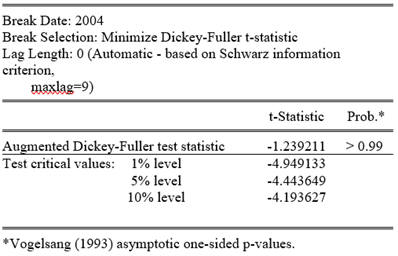
\includegraphics{Imagen12.png}

{\footnotesize Elaboración propia.}
\end{figure}

\begin{figure}[H]
\centering{5. Prueba de Bai-Perrón para determinar el número de raíces óptimo}
\par\vspace{0.8em}

\includegraphics{Imagen13.png}

{\footnotesize Elaboración propia.}

\end{figure}
\begin{figure}[H]
\centering{6. Resultados de aproximación trigonométrica de Fourier }
\par\vspace{0.8em}

\includegraphics{Imagen14.png}

{\footnotesize Elaboración propia. Nótese que aquí se uso la forma funcional siguiente: 
$y_t=α+β_t+ρy_{t-1}+δ⋅sin(\frac{2πt}{5})+θ⋅cos(\frac{2πt}{5})+\epsilon_t$. La finalidad fue hallar estacionalidad cada 5 años, de modo que fuese recurrente con las elecciones presidenciales. Aun tratando de hallar estacionalidad por 2, 3 o 4 años el resultado no es significativo. Para la elaboración, véase Seminario (2006) 
}
\end{figure}

\begin{figure}[H]
\centering{7. Resultados de poner los quiebres estructurales del Zivot-Andrews como explicativas en el ADF }
\par\vspace{0.8em}

\includegraphics{Imagen15.png}

{\footnotesize Elaboración propia. Nótese que el coeficiente de SERIES02(-1), que representa el primer rezago del gasto público, no es significativo. Esto es, la serie no se vuelve estacionaria. No se usa ningún rezago explicativo porque este estado minimiza los criterios de Schwartz y Akaike. La prueba, tanto en Zivot-Andrews como en Bai-Perron detectó a la tendencia del sistema como aquellas propias de los cambios de pendiente (quiebres en tendencia) como no significativas, por lo que se las excluyó de la prueba. }
\end{figure}

\begin{figure}[H]
\centering{8. Resultados de poner los quiebres estructurales del Bai-Perron como explicativas en el ADF }
\par\vspace{0.8em}

\includegraphics{Imagen16.png}

{\footnotesize Elaboración propia.}
\end{figure}


\end{document}